\documentclass{article}
\usepackage[paperheight=11in,paperwidth=8.5in,margin=1in]{geometry}
\usepackage{fancyhdr}
\usepackage{mdwlist}
\usepackage{graphicx}
\usepackage{tabularx}
\setlength{\headheight}{15.2pt}
\pagestyle{fancy}

\begin{document}
\newcommand{\lw}{Low}
\newcommand{\md}{Medium}
\newcommand{\hh}{High}
\fancyhf{}
\lhead{Team Security Crawler}
\chead{Final Project Design}
\rhead{\today}

\begin{titlepage}
\begin{center}
{\huge Team Security Crawler}\\[2cm]
{\Large Final Project Design}\\[2cm]
{\large \today}\\[2cm]
\emph{Team Members:}\\
Alex \uppercase{Audretsch}\\
Michael \uppercase{Eaton}\\
Trevor \uppercase{Krenz}\\
Andrew \uppercase{Siegle}\\[1cm]
\emph{Client:}\\
Alan WLASUK\\
WDDinc.\\[1cm]
\emph{Advisor:}\\
Steve CHENOWETH

\end{center}
\end{titlepage}
\tableofcontents
\newpage
\section{Introduction}

403 Security is a web security firm based out of Indianapolis that is looking to increase its client base by way of a free, automated security scan that a potential client can request by way of a web service.  This service will save 403 employees valuable time and generate a sizeable number of clients for 403.

To this end, the Security Crawler system has been designed.  Because it is an automated service that anyone can access, it is restricted to analysis of page source, and cannot perform in-depth penetration scans.  However, a sizeable number of security vulnerabilites can be deduced from this data, such as out-of-date software and bad permissions in the html file tree.

This document contains updated designs and architectural models for the security crawler system, as well as discussions of sysetm design choices in light of GRASP and GoF patterns.  It includes the logical architecture of the system and finally an integration and acceptance testing plan for the system when it is deployed.

\newpage
\section{Analysis Models}
\subsection{Domain Model}
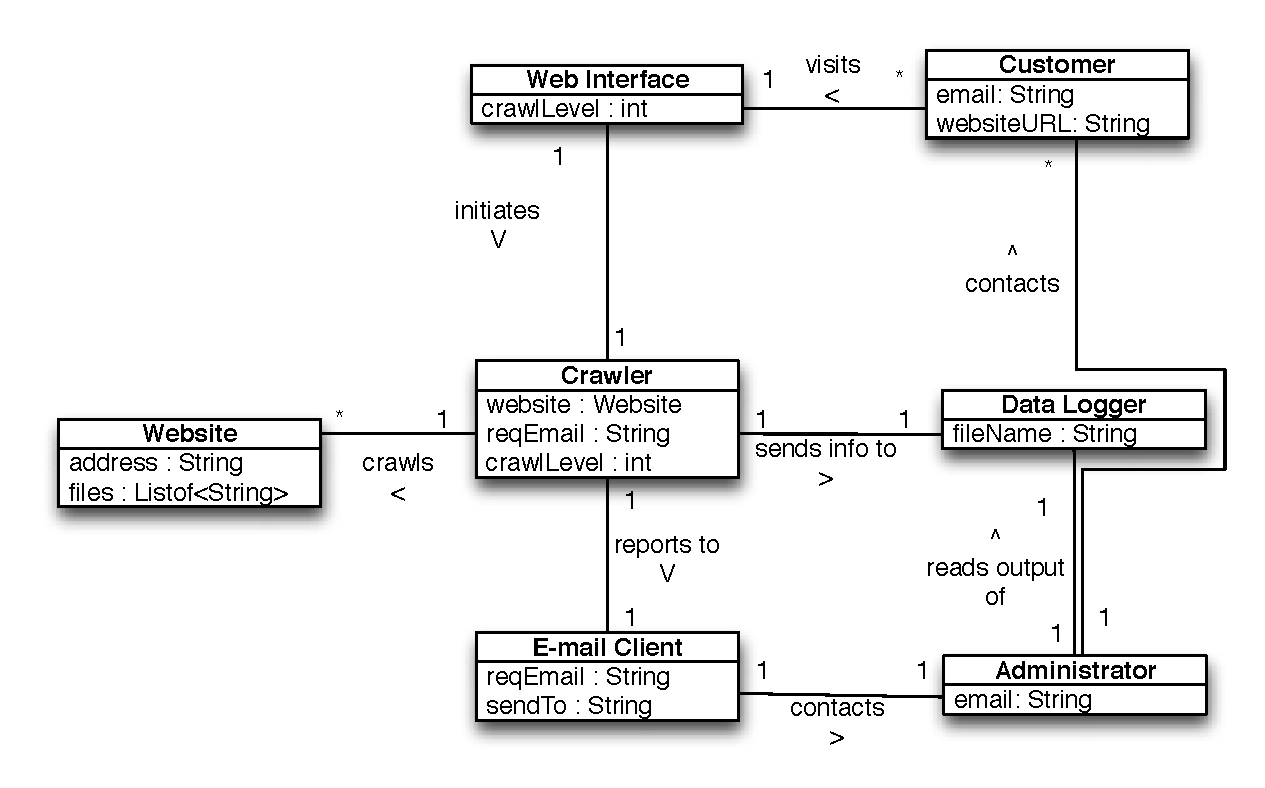
\includegraphics[width=\textwidth]{374DM.eps}
\subsection{System Sequence Diagram}
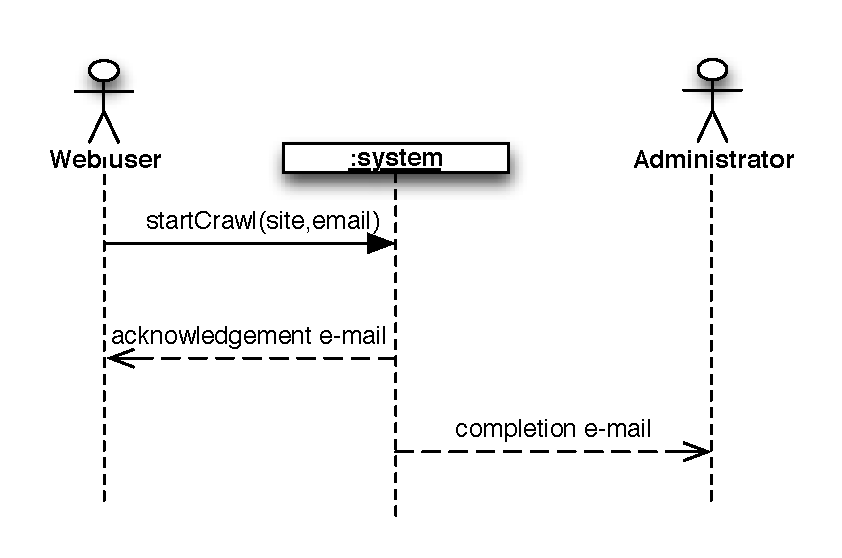
\includegraphics[width=\textwidth]{SSD}
\subsection{Sequence Diagrams}
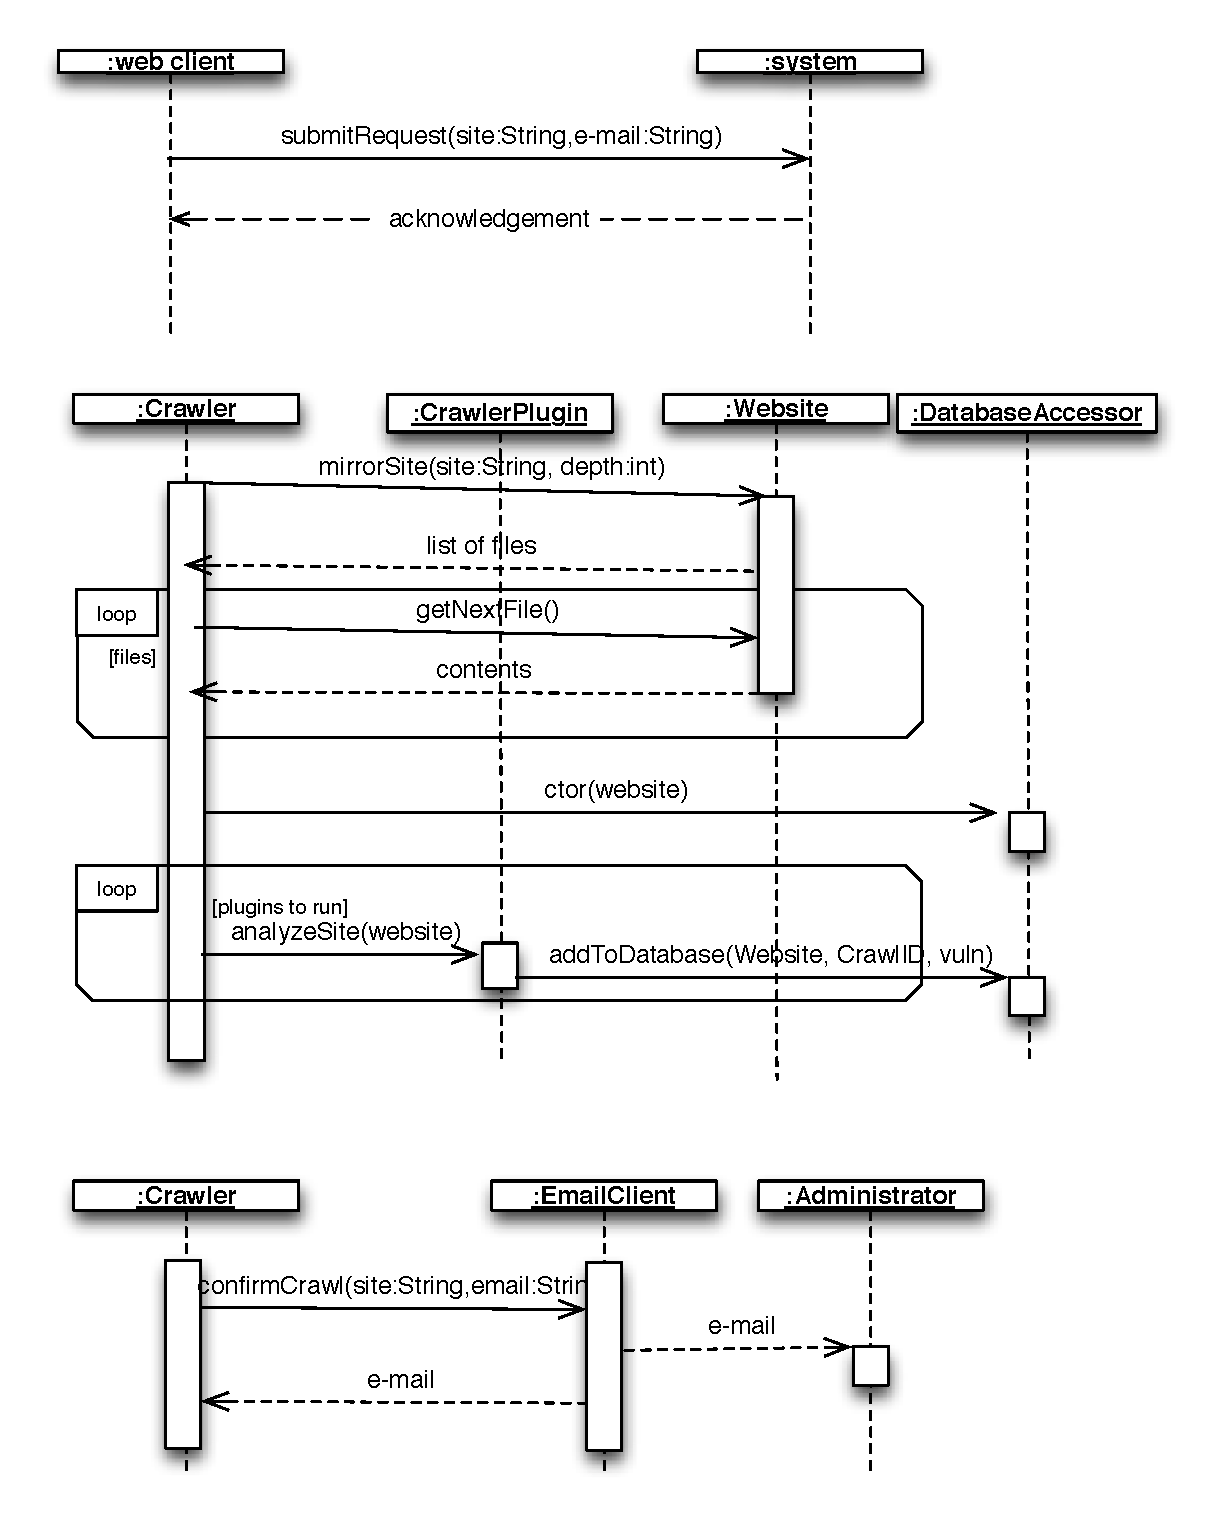
\includegraphics[width=\textwidth]{SeqDia}
\newpage
\subsection{Design Class Diagrams}
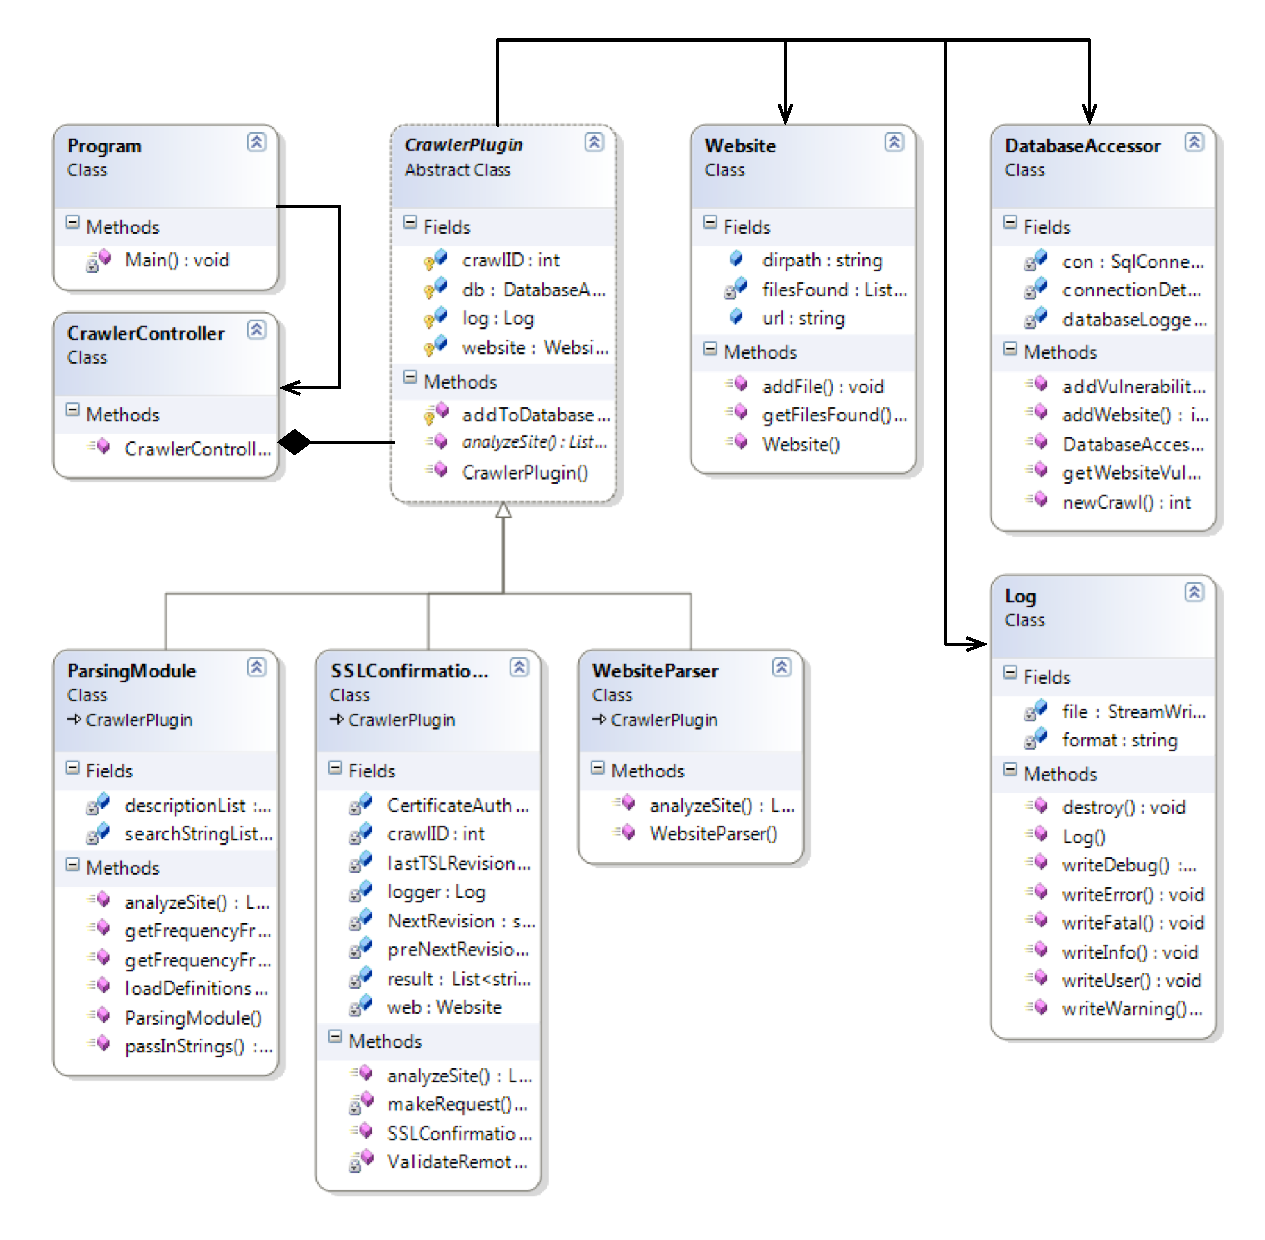
\includegraphics[width=\textwidth]{DCD}

\newpage
\subsection{Operations Contracts}
{\large \bf Contract 1:} mirrorSite \\[.5cm]
\begin{tabular}{|p{.2\textwidth} | p{.4\textwidth}|}
\hline
Operation: & crawlSite(address :string, level int) \\ \hline
Cross References: & Use Case: Initiate Web Crawl\\ \hline
Preconditions: &
\begin{itemize}
	\item Site address is known
	\item Site is valid
	\item There is enough space on the hard disk to store the contents of the website
\end{itemize}\\ \hline

Postconditions: &
\begin{itemize}
	\item The website has been mirrored the hard drive
	\item A list of all mirrored files is made
	\item A list of all vulnerabilities found has been made
\end{itemize}\\ \hline
\end{tabular} \\[1cm]

{\large \bf Contract 2:} compileVulnList\\[.5cm]
\begin{tabular}{|p{.2\textwidth} | p{.4\textwidth}|}
\hline
Operation: & compileVulnList() \\ \hline
Cross Reference: & Use Case: Display a Trace Log \\ \hline
Preconditions: & 
\begin{itemize}	
	\item All files have been parsed
	\item Certification and server information have been retrieved
	\item There is a List that contains all of the possible vulnerabilities to scan for
\end{itemize} \\ \hline

Postconditions:	&
\begin{itemize}
	\item A list of vulnerabilities is made
	\item The list of vulnerabilities are written to the database
	
\end{itemize} \\ \hline
\end{tabular}
\newpage
\section{Logical Architecture}
\includegraphics{LogArch}
\newpage
\section{Design with discussion}
\subsection{GRASP}
The \emph{CrawlerEngine} class follows the \textbf{Controller} GRASP principle. This is advantageous because the CrawlerEngine has the information needed to instantiate other classes, such as the website that is to be crawled (used to create a Website instance) and email address (for a EmailClient instance).\\\\% We thought that using a separate Controller class
The \emph{CrawlerEngine} is also uses the \textbf{Creator} principle. This makes handling passing the Log instance to all of the other classes easier, since the Log can be passed to all objects when they are instantiated, as opposed to the CrawlerEngine class being visible to the other classes and having to use methods to pass the Log object. Because the Log always becomes visible via the constructor of classes, coupling is decreased because the classes created by the CrawlerEngine class do not need visibility of CrawlerEngine. This also prevents circular references, which increases cohesion and decreases coupling.\\\\
Also, we have added a \emph{CrawlerPlugin} abstract class to our project. All plugins for the project will inherit from this class, and thus this is an example of \textbf{Polymorphism}. This increases cohesion because every class that inherits from the CrawlerPlugin class must override the methods in CrawlerPlugin, so it can be relied upon that all plugins can be interacted with via these methods. Additionally, the plugins for the crawler vary based on type, so it was a good idea to use polymorphism here.\\\\
The \emph{AbstractInferenceModule} is an example of \textbf{Pure Fabrication}. This is a class that does not exist in our domain model, but having this class increases cohesion and lowers coupling. For example, the CrawlerEngine already has the responsibility of creating other instances, and because of the Single Responsibility Principle, the responsibility of interpreting the should not be within this class. Instead, it is the responsibility of the AbstractInferenceModule to interpret the parsed results of the website.\\\\
By having the \emph{IInferenceModule} and the \emph{IInterfaceResult}, a level of \textbf{Indirection} was achieved. This increases cohesion because it makes the classes more closely adhere to the Single Responsibility Principle. Anything that has to deal with the results is in the IInterfaceResult, while the actual processing of documents is done by the IInferenceModule.\\\\
The \emph{server plugins} also demonstrate \textbf{Protected Variation}. Since this project is going to be taken over by another team once we are done, we know that it might change vastly, and the plugins for the crawler are points of instability. The class is then designed to handle plugins generally, which handles the instability.\\\\
The \emph{CrawlerEngine} is also an \textbf{Information Expert}. This follows naturally from it being a controller because it gets all of its information from the GUI. Having all of the data in one place and having the CrawlerEngine be responsible for the data will increase cohesion because it allows the other class to focus one responsibility, and do that responsibility well.\\\\

\subsection{Go4}
\textbf{Strategy} Our JavascriptLibrary object will contain some sort of identification strategy which will be injected into each object. We expect that we will need to compose some Javascript identification functions out of others, so in order to reuse code we’ll inject this behavior into each Javascript library we’re keeping track of.  This contrasts to something like ServerSoftware, whose relevant unique information would be HTTPHeader-related.\\\\
\textbf{Template Method} We may, in the future, compose the JavascriptLibrary identifier by templating a solution from a string-recognition function, a Javascript VM execution function, and a .js file handler. C\# is a functional language, so we can implement the functions directly, privately rather than making classes.\\\\
\textbf{Singleton} Our database adapter and email client classes are singletons. They network to outside sources, so we want to reduce the number of active connections as much as possible. In addition, our logger is currently only being instantiated once, but we’re injecting it into modules rather than making it static in case we want to refactor in the future and use several types of loggers.\\\\
\textbf{Adapter} Our two aforementioned singletons, database adapter and email client adapter, are adapters for .Net SQL and SMTP objects respectively. It’s obviously much easier on our part to have one-stop adapters than to worry about making the SQL- and email-handling objects directly.\\\\
\textbf{Iterator} Our CrawlEngine is an iterator on files it needs to analyze, using the GetNextFile() method. It will contain logic on which files to ignore and which to analyze while iterating (something like robots.txt would be ignored.)\\\\
\textbf{Template} The plugins follow the Gang of Four pattern of a template.  Each pluging implements its own version of analyzeSite which is then called from the CrawlerController class.  Each new plugin will follow this template in order to make creating new plugins easier.

\newpage
\section{Integration and Acceptance Test Plan}
\subsection{Current Status}
\subsubsection{Completed}
\begin{itemize}
	\item Database functionality - the database has been created on the school-hosted server with appropriate accounts.  Stored procedures are used to access the data.  A DatabaseAccessor class is present in the system as a singleton.
	\item Website mirroring - the system uses the external program 'HTTrack' to access the website and copy all available pages into a local directory in order to parse those files.  The files are saved in a directory named appropriatedly with the website and a timestamp.
	\item Basic parsing module - The basic parsing module reads a file of strings to look for in the files and scans them appropriately and records statistics according to frequency and also records vulnerabilities associated with the found contents.
	\item Framework - The system's basic framework and structure is laid down.  The Crawler acts as a controller and a factory, creating the needed plugins and running the analyseSite() method to invoke their functionality. 
\end{itemize}
\subsubsection{In Progress}
\begin{itemize}
	\item Server Info - Obtains server information by analyzing HTML headers and packets received by the crawler.
	\item SSL Certificate checking - Compare received SSL certificates to a known certificate authority in order to confirm validity.
	\item Script parsing - the system will be able to check for php, javascript...etc. vulnerabilities.
\end{itemize}
\subsubsection{To Do}
\begin{itemize}
	\item E-mail client - The system must send an e-mail to the administrator.
\end{itemize}
\subsection{Acceptance Test Plan}
For this project to be an acceptable success, it must be able to crawl a site, write to a database, and notifiy the administrator.  It must check SSL Certificates, retrieve server and website software packages and versions, and parse for basic javascript and php vulnerabilities.  The system also must be able to accept additional plugins for scanning various vulnerabilities, allowing for future expansions.

The system will be tested against a known security vulnerability scanner (Acunetix) in order to validate found vulnerabilities and  functionality.
\subsection{Required Features for Acceptance}
\begin{tabularx}{\textwidth}{|X|c|c|X|c|p{3.5cm}|}
	\hline
	\bf Feature &\bf Priority &\bf Version &\bf Reason &\bf Accepted & \bf Acceptance Criteria\\ \hline
	Parse / analyze HTML header information & Critical & v1.0 & Source of basic webpage and server data. & Yes & Output matches Acunetix output for at least 5 sites\\ \hline
	Examine server file tree & Critical & v1.0 & Potentially sensitive information may be hosted publicly. & Yes & Applicaiton mirrors complete site\\ \hline
	Save crawl results to database & Critical &v2.0 & Results must be saved for report generation and statistics tracking. & Yes & Vulnerability data saved successfuly to database\\ \hline
	Report crawl results & Critical &v1.0 & Results must be distributed to Alan so that he may report customized results to the user. & Yes & Email successfully delivered to admin-defined address\\ \hline
	Parse and analyze Javascript files & Critical & v3.0 & Javascript files are indicative of production framework. & Yes & Parse output matches basic Acunetix output\\ \hline
	Parse / analyze HTML form information & Important & v1.5  & Forms may indicate which framework generated them. & Yes & Output matches Acunetix output\\ \hline
	Examine site security certificates & Important & v2.0 & Check for expired certificates. & Yes & Expired and faulty certificates identified successfully\\ \hline
	Maintain operations tracelog & Important & v1.0 & Allows for traceback of operations for quality assurance and testing purposes. & Yes & All operations logged to acceptable detail level\\ \hline
	Basic Web GUI & Useful & v3.0 & Allows a user to enter information from client's web site. & No & User able to initiate a successful crawl via the web UI\\ \hline
	Compare previous crawl information & Useful & v3.0 & Allows the user to changes/improvements to website. & No & N/A \\ \hline
	Save search engine optimization (SEO) data & Useful & v3.0 & Retains information found during crawling for later statistical analysis on websites. & No & N/A\\ \hline
	Statistical analysis of crawls & Useful & v3.0 & Statistical tracking would give the client useful information about his or her website: how said site's vulnerabilities fit into the overall picture of web vulnerabilities, for example. & No & N/A\\ \hline
\end{tabularx}

\newpage
\section{Activity Diagram}
\includegraphics[width=.8\textwidth, scale=1]{activity1}

\includegraphics[width=.8\textwidth, scale=1]{activity2}

\newpage
\section{Who Done What Table}
\begin{center}
\begin{tabular}{|l|c|}
\hline
Team member & Tasks \\ \hline
Alex Audretsch & 
\begin{minipage}{.4\textwidth}
\vspace{11pt}
\begin{itemize}
	\item Updated DCD
	\item GoF Principles
\end{itemize} 
\end{minipage} \\ \hline
Michael Eaton & 
\begin{minipage}{.4\textwidth}
\vspace{11pt}
\begin{itemize}
	\item Introduction
	\item Logical Architecture
	\item Integration and Acceptance Plan
\end{itemize} 
\end{minipage} \\ \hline
Trevor Krenz & 
\begin{minipage}{.4\textwidth}
\vspace{11pt}
\begin{itemize}
	\item Design with explanation (GRASP and GoF Principles)
\end{itemize} 
\end{minipage} \\ \hline
Andrew Siegle & 
\begin{minipage}{.4\textwidth}
\vspace{11pt}
\begin{itemize}
	\item Document Design
	\item Sequence Diagrams
	\item Integration and Acceptance Plan
\end{itemize} 
\end{minipage} \\ \hline
\end{tabular}
\end{center}


\end{document}